\documentclass{article}

\usepackage[margin=1in]{geometry}
\usepackage{courier}
\usepackage{amsmath}
\usepackage{amssymb}
\usepackage{amsfonts}
\usepackage{bm}
\usepackage{enumitem}
\usepackage{wrapfig}
\usepackage{graphicx}
\usepackage[justification=centering]{subfig}
\usepackage{listings}
\usepackage{tikz}
\usepackage{pgf}
\usepackage{url}

\usepackage{booktabs,multirow}
\usetikzlibrary{arrows, automata}

\DeclareMathOperator*{\argmax}{arg\,max}
\DeclareMathOperator*{\argmin}{arg\,min}

\numberwithin{equation}{section}

\setlist[description]{leftmargin=\parindent,labelindent=\parindent}
\setlist[itemize,enumerate]{align=left}
\lstset{
	basicstyle=\ttfamily,
	tabsize=4,
	breaklines=true,
	linewidth=\linewidth
}
\setlength{\parindent}{0pt}

\title{01.112 Project}
\author{Gabriel Wong (1002299)
\and Lee Tze How (1002033) \and Koh Jing Yu (1002045)}

\begin{document}
\maketitle
\begin{abstract}
In this report, we document our code for the 01.112 project, as well as detail our experiments and approach for the design challenge. We use a multi-layer perceptron to achieve an entity F-score of 0.700 on EN and 0.677 on FR for the validation dataset.
\end{abstract}

\tableofcontents
\pagebreak

% \pagenumbering{gobble}
\setcounter{section}{1}

\section{Maximum Likelihood Estimation}
Our code for Part 2 is within the files \textit{Part2.py} and \textit{Part2.ipynb}.

\subsection{Emission Parameters Estimation} \label{sec:emissions}
In order to derive the count values, we process the file as follows.

Each line in the file represents a word followed by its label. For each label, we store the number of occurrences of each word in a dictionary with the key as the word, and the value as the number of occurrences. For a particular label, this results in a dictionary that looks something like the following:

\begin{verbatim}
{'Nous': 100, 'avons': 101, 'tout': 105, 'aimé': 7, '.': 1067, ... }
\end{verbatim}

We store this dictionary as the value of another dictionary, where the key represents the label. This results in the following dictionary:

\begin{verbatim}
emissions = {'B-negative': {'"': 1, 'Accueil': 7, 'Ambiance': 2, ...},
             'B-positive': { ... }, ... }
\end{verbatim}

This allows us to efficiently retrieve $\text{Count}(y \rightarrow x)$ using

\begin{verbatim}emissions[y][x]\end{verbatim}

Similarly, for computational efficiency, we store the counts of each label in a separate dictionary:

\begin{verbatim}
emission_counts = {'B-negative': 675, 'B-neutral': 113, 'B-positive': 810,
    'I-negative': 233, 'I-neutral': 43, 'I-positive': 181, 'O': 24512}
\end{verbatim}

We can then easily retrieve $\text{Count}(y)$ using

\begin{verbatim}emission_counts[x]\end{verbatim}

This allows us to efficiently retrieve the emission parameters $e(x|y)$, at the cost of a minor space complexity increase.

\subsection{Laplace Smoothing}

For smoothing, we implement a getter function for the emission parameters. If the given word $x$ does not exist in our parameters learnt from training data, we return the smoothed version of the parameters.

\begin{verbatim}
def get_emission_parameters(emissions, emission_counts, x, y, k=1):
    ''' Returns the MLE of the emission parameters based on the emissions dictionary '''
    state_data = emissions[y]
    count_y = emission_counts[y] #sum(state_data.values()) # Denominator
    
    # If x == "#UNK#", it will return the following
    count_y_x = k
    
    # If x exists in training, return its MLE instead
    if x != "#UNK#":
        count_y_x = state_data[x] # Numerator
    
    e = count_y_x / (count_y + k)
    return e{}
\end{verbatim}

\subsection{Sequence Labeling}

For sequence labeling, we implement a function that takes as input the sentence to be labeled, and the emission parameters as described in Section \ref{sec:emissions}:

\begin{verbatim}
def label_sequence(sentence, emissions, emission_counts):
    ''' Takes a list `sentence` that contains words of a sentence as strings '''
    tags = []
    
    for word in sentence:
        predicted_label = ""
        max_prob = -1
        
        # Find y with maximum probability
        for y in emissions:
            
            if word not in observations:
                word = "#UNK#"
            
            if (word in emissions[y]) or (word == "#UNK#"):
                prob = get_emission_parameters(emissions, emission_counts, word, y)
            
                # If this is higher than the previous highest, use this
                if prob > max_prob:
                    predicted_label = y
                    max_prob = prob

        # Add prediction to list
        tags.append(predicted_label)
    
    return tags
\end{verbatim}

For each word, it finds the $\argmax$ over $y$, and assigns this as the tag. The final output of this function is a list containing the predicted tags.

\subsection{Results}

Our results on the four datasets are as follows:

\begin{table}[htpb]
\centering
\begin{tabular}{|l|c|c|}
\hline
\multirow{2}{*}{\textbf{Dataset}} & \multicolumn{2}{c|}{\textbf{F-Score}} \\ \cline{2-3} 
 & \multicolumn{1}{l|}{\textbf{Entity}} & \multicolumn{1}{l|}{\textbf{\begin{tabular}[c]{@{}l@{}}Entity\\ Type\end{tabular}}} \\ \hline
EN & 0.6297 & 0.4595 \\ \hline
SG & 0.2952 & 0.1501 \\ \hline
CN & 0.1929 & 0.1134 \\ \hline
FR & 0.2751 & 0.1169 \\ \hline
\end{tabular}
\end{table}

\section{First-Order Hidden Markov Model}
\subsection{Transition Parameters Emission}
In order to derive the transition values, we process the file as follow.\\
Each line in the file represents a word followed by its label. For each label, we create a transition denoted by a tuple \lstinline{(previous label, current label)}. For the first and last label in each sentence, we also add the transitions \lstinline{(START, label)} and \lstinline{(label, STOP)} respectively. This results in a dictionary that looks something like the following.

\begin{verbatim}
{('START', 'O'): 1474, ('O', 'O'): 21452, ('O', 'STOP'): 1621, ...}
\end{verbatim}

In addition, for each tuple \lstinline{(a, b)} that we add to the dictionary, we also add the counts of \lstinline{a} and \lstinline{b} to a separate dictionary. This allows us to obtain the counts of each transition, as follows.

\begin{verbatim}
{'START': 1632, 'O': 24512, 'B-positive': 810, 'I-positive': 181,
    'B-negative': 675, 'B-neutral': 113, 'I-negative': 233, 'I-neutral': 43}
\end{verbatim}

This allows us to efficiently retrieve $\text{\lstinline{Count}}(y_{i-1}, y_i)$ and $\text{\lstinline{Count}}(y_{i-1})$, and obtain the transition parameters
	$$q(y_i | y_{i-1}) = \frac{\text{\lstinline{Count}}(y_{i-1}, y_i)}{\text{\lstinline{Count}}(y_{i-1})}$$
Note that \lstinline{STOP} is not necessary in the second dictionary, since there will never be a transition \emph{from} \lstinline{STOP}.

In addition, when $\text{\lstinline{Count}}(y^*_{i-1}) = 0$, we simply allow $q(y_i | y^*_{i-1}) = 0$.

\subsection{Viterbi Algorithm}
Combining Parts 2 and 3, we now have the estimated transition and emission parameters. We will denote them as
	$$ a_{u, v} = q(v | u) = \frac{\text{\lstinline{Count}}(u, v)}{\text{\lstinline{Count}}(u)} $$
	$$ b_u(x_j) = e(x | y) = \frac{\text{\lstinline{Count}}(u \rightarrow x_j)}{\text{\lstinline{Count}}(u)} $$

For each sequence , a \lstinline{pandas.DataFrame} object of size $\lvert\mathcal{T}\rvert \times (n+2)$ is used to store the probabilities of a given state at a given time, where $n$ is the length of the sequence, and $\mathcal{T}$ is the set of all states in training. $(n+2)$ is used to include the \lstinline{START} and \lstinline{STOP} observations as well.\\

Similarly, another \lstinline{pandas.DataFrame} object of the same size is created as a backpointer table to perform the backtracing algorithm. The probability table will be known as \lstinline{P} while the backpointer table will be known as \lstinline{B}.

\subsubsection{Initialization}
We begin by initializing $\pi(0, \text{\lstinline{START}}) = 1$.

\begin{verbatim}
    P.loc['START', 0] = 1
\end{verbatim}

\subsubsection{Recursion}
Next, as per the Viterbi algorithm:
	$$ \pi(j, v) = \max_{u\in\mathcal{T}} \{ \pi(j-1, u) \cdot a_{u, v} \cdot b_v(x_j) \}, \: \forall\; v \in \mathcal{T} $$
	
In addition, we also use the backpointer table to store the state transition $(y_{j-1}, y_j)$:
	$$\beta(j, v) = \argmax_{u\in\mathcal{T}} \{ \pi(j-1, u) \cdot a_{u, v} \cdot b_v(x_j) \}, \: \forall\; v \in \mathcal{T} $$
	
\begin{verbatim}
x_j = obs_seq[j-1]
for v in states:  # current state
    for u in states:  # previous state
        p = P.loc[u, j-1] * a(u, v) * b(v, x)
        if p > P.loc[v, j]:  # keep larger probability
        P.loc[v, j] = p  # update probability
        B.loc[v, j] = u  # update backpointer
\end{verbatim}

This operation is repeated for $j = \{1, ..., n+1\}$, where $x_{n+1} = \text{\lstinline{STOP}}$.

\subsubsection{Backtracking}
Finally, once the Viterbi algorithm is complete, we use the backpointer table to obtain the state sequence.
	$$ y_{n} = \beta(n+1, \text{\lstinline{STOP}}) $$
	$$ y_{j-1} = \beta(j, y_j),\; \forall\; j \in \{n-1, ..., 2, 1\} $$

The Python implementation of this is as follows:
\begin{verbatim}
state_seq = ['STOP']  # initialization
for i in range(n-1, 0, -1):  # {n-1, ..., 2, 1}
    curr_state = state_seq[-1]  # y_j
    prev_state = B.loc[curr_state, i]  # y_{j-1}
    state_seq.append(prev_state)
\end{verbatim}

In special cases where there is no observed transition (i.e. $P(y_{j-1} | y_j) = 0$), we might obtain an observation sequence $x_1, x_2, ..., x_n$ that has a probability of $0$. In this scenario, we simply predict a sequence of \lstinline{O}'s.

\subsection{Results}
Our results on the four datasets are as follows:

\begin{table}[htpb]
	\centering
	\begin{tabular}{|l|c|c|}
		\hline
		\multirow{2}{*}{\textbf{Dataset}} & \multicolumn{2}{c|}{\textbf{F-Score}} \\ \cline{2-3} 
		& \multicolumn{1}{l|}{\textbf{Entity}} & \multicolumn{1}{l|}{\textbf{\begin{tabular}[c]{@{}l@{}}Entity\\ Type\end{tabular}}} \\ \hline
		EN & 0.6379 & 0.5556 \\ \hline
		SG & 0.4185 & 0.2531 \\ \hline
		CN & 0.3955 & 0.2700 \\ \hline
		FR & 0.3994 & 0.2232 \\ \hline
	\end{tabular}
\end{table}

\section{Second-Order Hidden Markov Model}


\section{Design Challenge}
\subsection{Preprocessing}
\subsubsection{String tokenization}
Each file can be considered a corpus, the documents being each sentence in the file. Tokenizing was carried out by converting each sentence into a list of words. During tokenization, all whitespace was stripped from the beginning and end of each word. Also, each token is normalized by converting to lowercase.

\subsubsection{Replacing irrelevant words}
In the initial problem, the training data contains a large vocabulary of words which occurred only a single time. To mitigate this issue, several types of words were converted into various placeholders instead, as they do not carry semantic meaning. \\

The placeholders used are as follows:
\begin{enumerate}
	\item \lstinline{#PUNC#}: strings that do not contain alphanumeric characters
	\item \lstinline{#HASH#}: hashtags (strings beginning with a \lstinline{#} character)
	\item \lstinline{#AT#}: \lstinline{@} mentions (strings beginning with a \lstinline{@} character)
	\item \lstinline{#NUM#}: strings that contain only digits
	\item \lstinline{#URL#}: strings that begin with \lstinline{http:} and end with \lstinline{.com}
\end{enumerate}

\subsubsection{Stop words}
Stop words were also initially converted to a token labeled \lstinline{#STOP#}. However, during evaluation on the \lstinline{EN} and \lstinline{SG} dataset with Part 3, it was shown to reduce the $F_1$ score on both the \emph{Correct Entity} and \emph{Correct Entity Type} tasks. It was also shown to produce poorer $F_1$ scores on the \lstinline{EN} dataset with Part 5. \\

Taking into account the negative correlation between removing stop words and $F_1$ scores, as well as the fact that we do not have French stop words, we decided not to remove stop words from the training data.


\subsection{Simple vectorization}
We discuss an implementation to convert each word into a vector, allowing us to train a recurrent neural network (RNN) with the text sequences.

\subsubsection{Tokenizing}
Tokenizing transforms each text into a sequence of integers, which allows us to vectorize the text corpus.\\

We first obtain a vocabulary of all unique words that have appeared in the training data.  We then assign a unique integer to each word, as well as 1 additional integer for the \lstinline{#UNK#} token, which denotes words not present in the vocabulary.

\begin{verbatim}
{'rt': 0,
 '#AT#': 1,
 '#PUNC#': 2,
 'encore': 3,
 ...,
 'bpa': 2502,
 '#UNK#': 2503}
\end{verbatim}

The following is a sample output sequence that has been tokenized:
\begin{verbatim}
# input: 'rt #AT# #PUNC# encore #PUNC# #AT# for ... #PUNC#'
[ 0,  1,  2,  3,  2,  1,  4,  ...,  2]
\end{verbatim}

\subsubsection{One-hot encoding}
Once each word has been converted into a corresponding integer, each integer is then converted into a vector via one-hot encoding.\\

Let $\mathcal{V}$ be the set of all words in the training vocabulary, including \lstinline{#UNK#}. Then, one-hot encoding maps each input to a vector, $f: \mathbb{R} \rightarrow \mathbb{R}^{|\mathcal{V}|}$.
	$$ f(n)_i = \left\{\begin{matrix}
	1, \; \text{if } i=n\\ 
	0, \; \text{otherwise}
	\end{matrix}\right. $$

\subsection{word2vec}
\emph{word2vec} is used as a feature extraction method, to convert the sparse one-hot encoding into dense vectors.

\subsubsection{Skip-gram}
A skip-gram architecture with a window size of $5$ is used for the training of the \emph{word2vec}. This means that given a sequence of words $\bm{x}^{(1)}, \bm{x}^{(2)}, ..., \bm{x}^{(n)}$, for an input variable $\bm{x}^{(i)}$, the target variable $\bm{y}^{(i)} \in \{\bm{x}^{(i-2)}, \bm{x}^{(i-1)}, \bm{x}^{(i+1)}, \bm{x}^{(i+2)}\}$.\\

We initialize two sets of weights, $\bm{W} \in \mathbb{R}^{300 \times |\mathcal{V}|}$ and $\bm{U} \in \mathbb{R}^{|\mathcal{V}| \times 300}$, with each value drawn from a normal distribution $\mathcal{N} \sim (0, 0.1^2)$.\\

\subsubsection{Forward}
The model is defined as such:
\begin{equation}
\begin{split}
	\bm{x}^{(i)}, \bm{y}^{(i)} &\in \mathbb{R}^{|\mathcal{V}|} \\
	\bm{h}^{(i)} &= \bm{W} \bm{x}^{(i)} \\
	\bm{o}^{(i)} &= \bm{U} \bm{h}^{(i)} \\
 	\hat{\bm{y}}^{(i)} &= \text{softmax}(\bm{o}^{(i)}) \\
	\mathcal{L} &= -\sum_{y^{(i)}} \bm{y}^{(i)} \cdot \text{log}(\hat{\bm{y}}^{(i)})
\end{split}
\end{equation}

The loss function is the sum of the cross-entropy loss between all target variables in the context, and the predicted variable.

\subsubsection{Backward}
\begin{equation}
\begin{split}
\frac{\partial \mathcal{L}^{(i)}}{\partial \bm{o}^{(i)}}
	&= \text{softmax}(\bm{o}^{(i)}) - \bm{y}^{(i)} \\
	&= \hat{\bm{y}}^{(i)} - \bm{y}^{(i)}
\end{split}
\end{equation}

\begin{equation}
\begin{split}
\frac{\partial \mathcal{L}^{(i)}}{\partial \bm{U}}
	&= \frac{\partial \mathcal{L}^{(i)}}{\partial \bm{o}^{(i)}} \frac{\partial \bm{o}^{(i)}}{\partial \bm{U}} \\
	&= (\hat{\bm{y}}^{(i)} - \bm{y}^{(i)}) \bm{h}^{(i)^T}
\end{split}
\end{equation}

\begin{equation}
\begin{split}
\frac{\partial \mathcal{L}^{(i)}}{\partial \bm{h}^{(i)}}
	&= \frac{\partial \mathcal{L}^{(i)}}{\partial \bm{o}^{(i)}} \frac{\partial \bm{o}^{(i)}}{\partial \bm{h}^{(i)}} \\
	&= \bm{U}^T(\hat{\bm{y}}^{(i)} - \bm{y}^{(i)})
\end{split}
\end{equation}

\begin{equation}
\begin{split}
\frac{\partial \mathcal{L}^{(i)}}{\partial \bm{W}}
	&= \frac{\partial \mathcal{L}^{(i)}}{\partial \bm{h}^{(i)}} \frac{\partial \bm{h}^{(i)}}{\partial \bm{W}} \\
	&= \bm{U}^T(\hat{\bm{y}}^{(i)} - \bm{y}^{(i)}) \bm{x}^{(i)^T}
\end{split}
\end{equation}

\subsubsection{Training}
\paragraph{Positive sampling}\mbox{}\\
For each word in every sentence, we take that word to be the center word. Then, for each word in its context, we update the weights according to the equations above.

\paragraph{Negative sampling}\mbox{}\\
For each word in every sentence, we take that word to be the center word. We also obtain the context words. Next, we sample 20 words from the vocabulary, excluding the center and context words, as recommended for small datasets \cite{DBLP:journals/corr/MikolovSCCD13}. The probability of sampling a word $w$ is given by the following equation, to reduce the probability of oversampling frequent words:
	$$ P(w) = \frac{\text{Count}(w)^\frac{3}{4}}{\sum_{w'}(\text{Count}(w')^\frac{3}{4})}  $$
	
The corresponding loss function for the negative samples is then given by:
	$$ \mathcal{L} = -\sum_{y^{(i)}} -\bm{y}^{(i)} \cdot \text{log}(\hat{\bm{y}}^{(i)}) $$

\subsubsection{Visualization}
We use t-SNE to reduce each word vector to 2 dimensions for visualization.\\
The results are shown in Figure \ref{fig:word2vec}.

\begin{figure}[h]
	\centering
	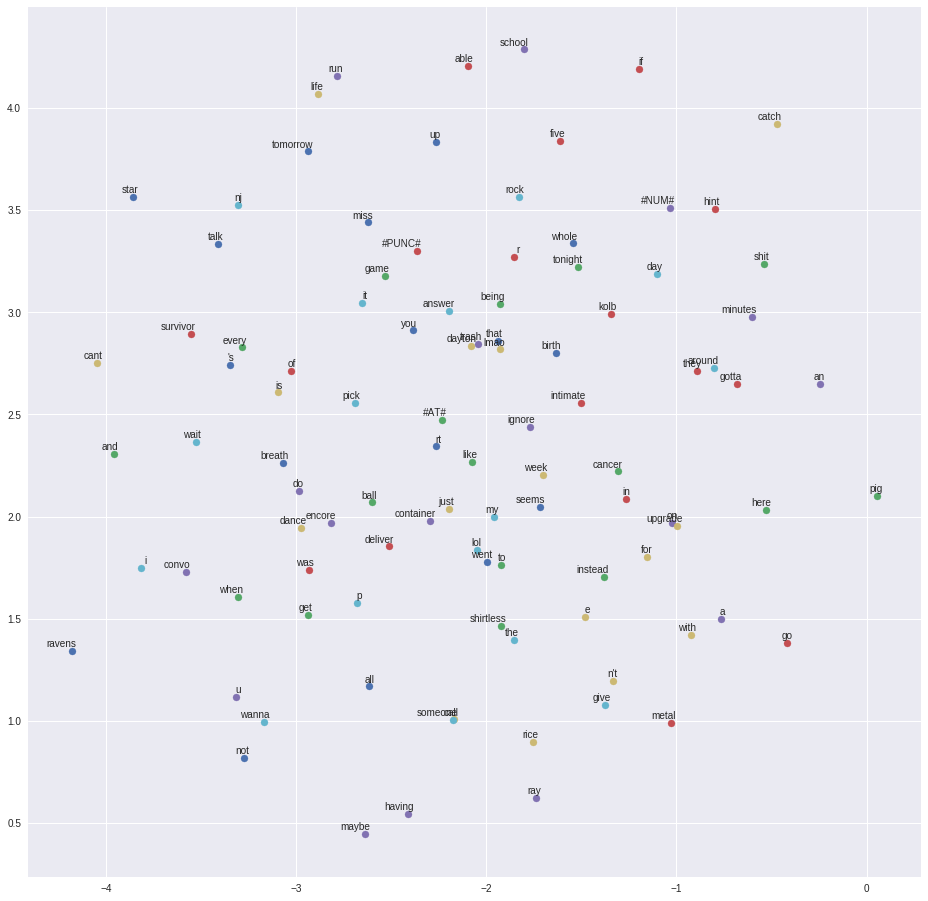
\includegraphics[width=0.9\linewidth]{assets/word2vec.png}
	\caption{t-SNE visualization of \emph{word2vec} model on EN dataset}
	\label{fig:word2vec}
\end{figure}

\subsubsection{Inference}
During inference, both weights $\bm{W}, \bm{U}$ are combined via averaging \cite{pennington2014glove}.
	$$ \bm{h} = \frac{1}{2}(\bm{W} + \bm{U}^T) \bm{x} $$

It is also common to find words in the validation and test sets that are not found in the training set. As such, these words are not in the \emph{word2vec} vocabulary. \\

Instead of simply treating these words as an \lstinline{#UNK#} token, they were represented as the mean of their context, within a window of size 5.
	$$ x_i = \frac{1}{4}(x_{i-2} + x_{i-1} + x_{i+1} + x_{i+2}) $$

\subsection{Recurrent neural network (RNN)}
\subsubsection{Forward}
We use a RNN, with a computational graph as shown in Figure \ref{fig:rnn}. The RNN maps an input sequence $\bm{x}$ to an output sequence $\bm{o}$. The predicted labels are then given by $\hat{\bm{y}} = \text{softmax}(\bm{o})$.\\

\begin{figure}[h!]
	\centering
	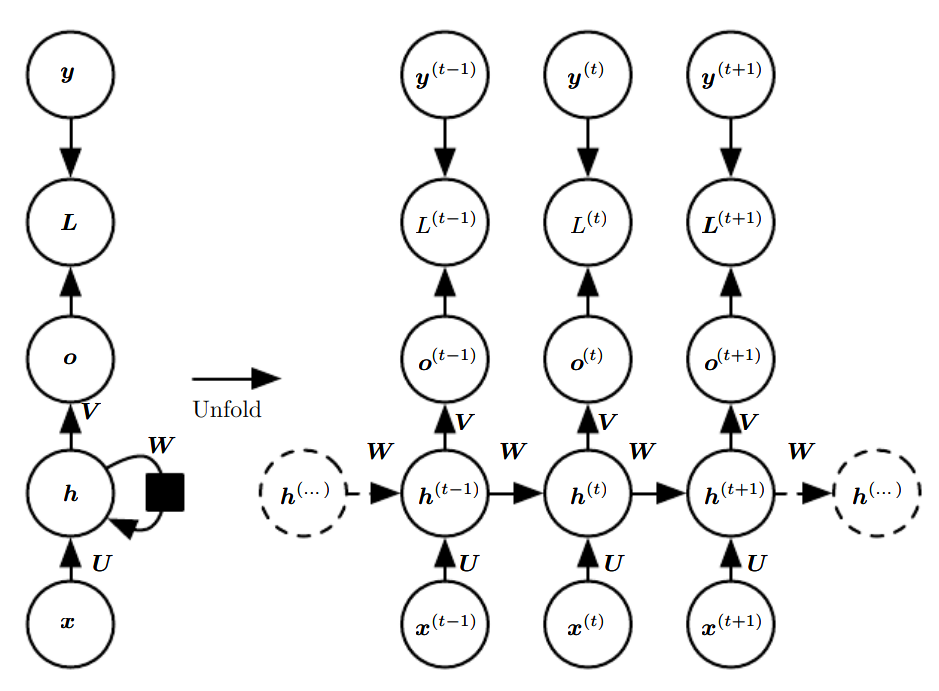
\includegraphics[width=0.7\linewidth]{assets/rnn.png}
	\caption{RNN model architecture \cite{Goodfellow-et-al-2016}}
	\label{fig:rnn}
\end{figure}

The loss function $\mathcal{L}$ compares the predicted labels $\hat{\bm{y}}$ with the target labels $\bm{y}$ through cross-entropy loss, where $C$ is the number of classes in the classification task.
	$$ \mathcal{L} = -\sum_i^C \bm{y}_i \cdot \text{log}(\hat{\bm{y}}_i) $$

The remaining nodes in the graph are computed as shown in Equation \ref{eqn:forward-all}.
\begin{equation}
\label{eqn:forward-all}
\begin{split}
	\bm{a}^{(t)} &= \bm{b} + \bm{U}\bm{x}^{(t)} + \bm{W}\bm{h}^{(t-1)} \\
	\bm{h}^{(t)} &= \text{tanh}(\bm{a}^{(t)}) \\
	\bm{o}^{(t)} &= \bm{c} + \bm{V}\bm{h}^{(t)} \\
	\hat{\bm{y}}^{(t)} &= \text{softmax}(\bm{o}^{(t)})
\end{split}
\end{equation}

$\bm{U}, \bm{W}, \bm{V}$ are the weight matrices, while $\bm{b}, \bm{c}$ are biases. By choice of hyperparameters, $\bm{h}^{(t)} \in \mathbb{R}^{128\times1}$. \\

For an input sequence, $\bm{x}^{(1)}, \bm{x}^{(2)}, ..., \bm{x}^{(n)}$, we first compute the hidden units $\bm{h}^{(t)}$ as shown in Equation \ref{eqn:forward-h}. At $t=1$, the hidden unit is computed using only $x^{(1)}$. Once we have the value of $\bm{h}^{(t)}$, we can then compute its predicted state $\hat{\bm{y}}^{(t)}$ with Equation \ref{eqn:forward-all}.

\begin{equation}
\label{eqn:forward-h}
\begin{split}
	\bm{h}^{(1)} &= \text{tanh}(\bm{b} + \bm{U}\bm{x}^{(1)}) \\
	\bm{h}^{(t)} &= \text{tanh}(\bm{b} + \bm{U}\bm{x}^{(t)} + \bm{W}\bm{h}^{(t-1)}),\;
		\forall\: t \in \{2, ..., n\}
\end{split}
\end{equation}

\subsubsection{Backward}
To perform backpropagation, our objective is to obtain the partial differential of $\mathcal{L}$ with respect to the weights and biases. The gradients are taken to be the \textbf{sum} over all time steps $t \in \{1, ..., n\}$.

\paragraph{Output layer}
\begin{equation}
\label{eqn:backward-o}
\begin{split}
	\frac{\partial \mathcal{L}^{(t)}}{\partial \bm{o}^{(t)}}
		&= \text{softmax}(\bm{o}^{(t)}) - \bm{y}^{(t)} \\
		&= \hat{\bm{y}}^{(t)} - \bm{y}^{(t)}
\end{split}
\end{equation}

\begin{equation}
\label{eqn:backward-c}
\begin{split}
	\frac{\partial \mathcal{L}}{\partial \bm{c}}
		&= \sum_{t=1}^n \frac{\partial \mathcal{L}^{(t)}}{\partial \bm{o}^{(t)}} \frac{\partial \bm{o}^{(t)}}{\partial \bm{c}} \\
		&= \sum_{t=1}^n (\hat{\bm{y}}^{(t)} - \bm{y}^{(t)}) \frac{\partial(\bm{c} + \bm{V}\bm{h}^{(t)})}{\partial \bm{c}} \\
		&= \sum_{t=1}^n (\hat{\bm{y}}^{(t)} - \bm{y}^{(t)})
\end{split}
\end{equation}

\begin{equation}
\label{eqn:backward-V}
\begin{split}
	\frac{\partial \mathcal{L}}{\partial \bm{V}}
		&= \sum_{t=1}^n \frac{\partial \mathcal{L}^{(t)}}{\partial \bm{o}^{(t)}} \frac{\partial \bm{o}^{(t)}}{\partial \bm{V}} \\
		&= \sum_{t=1}^n (\hat{\bm{y}}^{(t)} - \bm{y}^{(t)}) \frac{\partial(\bm{c} + \bm{V}\bm{h}^{(t)})}{\partial \bm{V}} \\
		&= \sum_{t=1}^n (\hat{\bm{y}}^{(t)} - \bm{y}^{(t)}) \; \bm{h}^{(t)^T}
\end{split}
\end{equation}

\paragraph{Hidden layer}\mbox{}\\
To compute the gradients of the hidden units $\frac{\partial \mathcal{L}}{\partial \bm{h}^{(t)}}$, we initialize the gradient at $t = n$, since it has no subsequent time step, and its gradient is dependent only on $\bm{o}^{(n)}$.

\begin{figure}[h!]
\centering
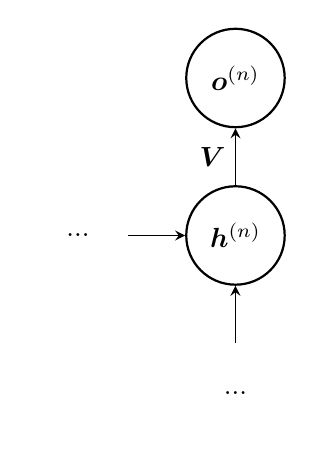
\begin{tikzpicture}[>=stealth, auto, node distance=2cm, semithick]
\tikzstyle{every state}=[draw=black, thick, fill=white, minimum size=1.25cm]

\node[state] (hn) {$\bm{h}^{(n)}$};
\node[state] (on) [above of=hn] {$\bm{o}^{(n)}$};
\node[state][draw=white] (ht) [left of=hn] {...};
\node[state][draw=white] (xt) [below of=hn] {...};

\path[->] (xt) edge node {} (hn);
\path[->] (ht) edge node {} (hn);
\path[->] (hn) edge node {$\bm{V}$} (on);
\end{tikzpicture}
\caption{Computational graph showing gradients for $\bm{h}^{(n)}$}
\label{fig:grad-hn}
\end{figure}

\begin{equation}
\label{eqn:backward-hn}
\begin{split}
	\frac{\partial \mathcal{L}^{(n)}}{\partial \bm{h}^{(n)}}
		&= \frac{\partial \mathcal{L}^{(n)}}{\partial \bm{o}^{(n)}} \frac{\partial \bm{o}^{(n)}}{\partial \bm{h}^{(n)}} \\
		&= (\hat{\bm{y}}^{(n)} - \bm{y}^{(n)}) \frac{\partial(\bm{c} + \bm{V}\bm{h}^{(n)})}{\partial \bm{h}^{(n)}} \\
		&= \bm{V}^T(\hat{\bm{y}}^{(n)} - \bm{y}^{(n)})
\end{split}
\end{equation}

Now, we can formulate the rest of the gradients recursively.

\begin{figure}[h!]
\centering
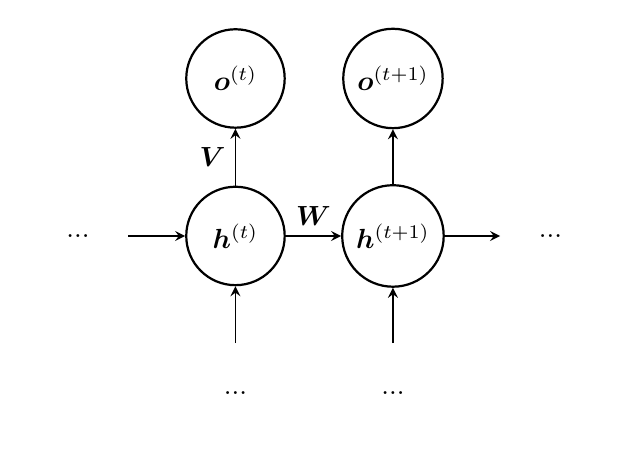
\begin{tikzpicture}[>=stealth, auto, node distance=2cm, semithick]
\tikzstyle{every state}=[draw=black, thick, fill=white, minimum size=1.25cm]

\node[state] (ht) {$\bm{h}^{(t)}$};
\node[state] (ot) [above of=ht] {$\bm{o}^{(t)}$};
\node[state] (ht+1) [right of=ht]{$\bm{h}^{(t+1)}$};
\node[state] (ot+1) [above of=ht+1] {$\bm{o}^{(t+1)}$};
\node[state][draw=white] (ht-1) [left of=ht] {...};
\node[state][draw=white] (xt) [below of=ht] {...};
\node[state][draw=white] (ht+2) [right of=ht+1] {...};
\node[state][draw=white] (xt+1) [below of=ht+1] {...};

\path[->] (xt) edge node {} (ht);
\path[->] (xt+1) edge node {} (ht+1);

\path[->] (ht-1) edge node {} (ht);
\path[->] (ht) edge node {$\bm{W}$} (ht+1);
\path[->] (ht+1) edge node {} (ht+2);

\path[->] (ht) edge node {$\bm{V}$} (ot);
\path[->] (ht+1) edge node {} (ot+1);
\end{tikzpicture}
\caption{Computational graph showing gradients for $\bm{h}^{(t)}$}
\label{fig:grad-ht}
\end{figure}

	$$ \frac{\partial \mathcal{L}^{(t)}}{\partial \bm{h}^{(t)}}
		= \frac{\partial \mathcal{L}^{(t)}}{\partial \bm{o}^{(t)}} \frac{\partial \bm{o}^{(t)}}{\partial \bm{h}^{(t)}}
		+ \frac{\partial \mathcal{L}^{(t+1)}}{\partial \bm{h}^{(t+1)}} \frac{\partial \bm{h}^{(t+1)}}{\partial \bm{h}^{(t)}} $$

From the result in Equation \ref{eqn:backward-hn}, we have that
	$$ \frac{\partial \mathcal{L}^{(t)}}{\partial \bm{o}^{(t)}} \frac{\partial \bm{o}^{(t)}}{\partial \bm{h}^{(t)}}
		 = \bm{V}^T(\hat{\bm{y}}^{(t)} - \bm{y}^{(t)}) $$

\begin{equation*}
\begin{split}
	\frac{\partial \mathcal{L}^{(t+1)}}{\partial \bm{h}^{(t+1)}} \frac{\partial \bm{h}^{(t+1)}}{\partial \bm{h}^{(t)}}
		&= \frac{\partial \mathcal{L}^{(t+1)}}{\partial \bm{h}^{(t+1)}} \frac{\partial \bm{h}^{(t+1)}}{\partial \bm{a}^{(t+1)}} \frac{\partial \bm{a}^{(t+1)}}{\partial \bm{h}^{(t)}} \\
		&= \frac{\partial \mathcal{L}^{(t+1)}}{\partial \bm{h}^{(t+1)}} \frac{\partial( \text{tanh}(\bm{a}^{(t+1)}))}{\partial \bm{a}^{(t+1)}} \frac{\partial (\bm{b} + \bm{U}\bm{x}^{(t+1)} + \bm{W}\bm{h}^{(t)})}{\partial \bm{h}^{(t)}} \\
		&= \bm{W}^T \frac{\partial \mathcal{L}^{(t+1)}}{\partial \bm{h}^{(t+1)}} \frac{\partial( \text{tanh}(\bm{a}^{(t+1)}))}{\partial \bm{a}^{(t+1)}} \\
		&= \bm{W}^T \text{diag}(1 - (\bm{h}^{(t+1)})^2) \frac{\partial \mathcal{L}^{(t+1)}}{\partial \bm{h}^{(t+1)}}
\end{split}
\end{equation*}

Combining the above results, we obtain
\begin{equation}
\label{eqn:backward-ht}
\begin{split}
	\frac{\partial \mathcal{L}^{(t)}}{\partial \bm{h}^{(t)}}
		&= \frac{\partial \mathcal{L}^{(t)}}{\partial \bm{o}^{(t)}} \frac{\partial \bm{o}^{(t)}}{\partial \bm{h}^{(t)}} 
			+ \frac{\partial \mathcal{L}^{(t+1)}}{\partial \bm{h}^{(t+1)}} \frac{\partial \bm{h}^{(t+1)}}{\partial \bm{h}^{(t)}} \\
		&= \bm{V}^T(\hat{\bm{y}}^{(t)} - \bm{y}^{(t)}) + \bm{W}^T \text{diag}(1 - (\bm{h}^{(t+1)})^2) \frac{\partial \mathcal{L}}{\partial \bm{h}^{(t+1)}}
\end{split}
\end{equation}\\

It is next imperative to show that the Jacobian $J^{(t+1)} = \frac{\partial \bm{h}^{(t+1)}}{\partial \bm{a}^{(t+1)}} = \frac{\partial( \text{tanh}(\bm{a}^{(t+1)}))}{\partial \bm{a}^{(t+1)}} = \text{diag}(1 - (\bm{h}^{(t+1)})^2)$. \\

We begin with the knowledge that $\frac{d}{dx}\text{tanh}(x) = 1 - \text{tanh}^2(x)$.
	$$ J^{(t+1)}_{ij} = \frac{\partial \bm{h}^{(t+1)}_i}{\partial \bm{a}^{(t+1)}_j} $$
For $i \ne j$, $J^{(t)}_{ij} = 0$. \\
For $i = j$,
\begin{equation*}
\begin{split}
	J^{(t+1)}_{ii} = \frac{\partial \bm{h}^{(t+1)}_i}{\partial \bm{a}^{(t+1)}_i} 
		&= \frac{\partial( \text{tanh}(\bm{a}^{(t+1)})_i)}{\partial \bm{a}^{(t+1)}_i} \\
		&= 1 - \text{tanh}^2 (\bm{a}^{(t+1)})_i \\
		&= 1 - (\bm{h}^{(t+1)}_i)^2
\end{split}
\end{equation*}

	$$ \therefore J^{(t)} = \frac{\partial \bm{h}^{(t)}}{\partial \bm{a}^{(t)}} =
		\begin{pmatrix}
		1 - (\bm{h}_1^{(t)})^2 & 0 & ... & 0 \\ 
		0 & 1 - (\bm{h}_2^{(t)})^2 & ... & 0 \\ 
		... & ... & 1 - (\bm{h}_i^{(t)})^2 & ... \\ 
		0 & 0 & ... & 1 - (\bm{h}_n^{(t)})^2
		\end{pmatrix} 
		= \text{diag}(1 - (\bm{h}^{(t)})^2) $$\\


We can then use this result to obtain the gradients with respect to $\bm{b}, \bm{W}, \bm{U}$.
\begin{equation}
\label{eqn:backward-b}
\begin{split}
	\frac{\partial \mathcal{L}}{\partial \bm{b}}
		&= \sum_{t=1}^{n} \frac{\partial \mathcal{L}^{(t)}}{\partial \bm{h}^{(t)}} \frac{\partial \bm{h}^{(t)}}{\partial \bm{a}^{(t)}} \frac{\partial \bm{a}^{(t)}}{\partial \bm{b}} \\
		&= \sum_{t=1}^{n} \text{diag}(1 - (\bm{h}^{(t)})^2) \frac{\partial \mathcal{L}^{(t)}}{\partial \bm{h}^{(t)}} \frac{\partial (\bm{b} + \bm{U}\bm{x}^{(t)} + \bm{W}\bm{h}^{(t-1)})}{\partial \bm{b}} \\
		&= \sum_{t=1}^{n} \text{diag}(1 - (\bm{h}^{(t)})^2) \frac{\partial \mathcal{L}^{(t)}}{\partial \bm{h}^{(t)}}
\end{split}
\end{equation}

\begin{equation}
\label{eqn:backward-W}
\begin{split}
	\frac{\partial \mathcal{L}}{\partial \bm{W}}
		&= \sum_{t=1}^{n} \frac{\partial \mathcal{L}^{(t)}}{\partial \bm{h}^{(t)}} \frac{\partial \bm{h}^{(t)}}{\partial \bm{a}^{(t)}} \frac{\partial \bm{a}^{(t)}}{\partial \bm{W}} \\
		&= \sum_{t=1}^{n} \text{diag}(1 - (\bm{h}^{(t)})^2) \frac{\partial \mathcal{L}^{(t)}}{\partial \bm{h}^{(t)}} \frac{\partial (\bm{b} + \bm{U}\bm{x}^{(t)} + \bm{W}\bm{h}^{(t-1)})}{\partial \bm{W}} \\
		&= \sum_{t=1}^{n} \text{diag}(1 - (\bm{h}^{(t)})^2) \frac{\partial \mathcal{L}^{(t)}}{\partial \bm{h}^{(t)}} \bm{h}^{(t-1)^T}
\end{split}
\end{equation}

\begin{equation}
\label{eqn:backward-U}
\begin{split}
	\frac{\partial \mathcal{L}}{\partial \bm{U}}
		&= \sum_{t=1}^{n} \frac{\partial \mathcal{L}^{(t)}}{\partial \bm{h}^{(t)}} \frac{\partial \bm{h}^{(t)}}{\partial \bm{a}^{(t)}} \frac{\partial \bm{a}^{(t)}}{\partial \bm{U}} \\
		&= \sum_{t=1}^{n} \text{diag}(1 - (\bm{h}^{(t)})^2) \frac{\partial \mathcal{L}^{(t)}}{\partial \bm{h}^{(t)}} \frac{\partial (\bm{b} + \bm{U}\bm{x}^{(t)} + \bm{W}\bm{h}^{(t-1)})}{\partial \bm{U}} \\
		&= \sum_{t=1}^{n} \text{diag}(1 - (\bm{h}^{(t)})^2) \frac{\partial \mathcal{L}^{(t)}}{\partial \bm{h}^{(t)}} \bm{x}^{(t)^T}
\end{split}
\end{equation}

\paragraph{Summary}
\begin{equation}
\label{eqn:backward-all}
\begin{split}
	\frac{\partial \mathcal{L}}{\partial \bm{U}}
		&= \sum_{t=1}^{n} \text{diag}(1 - (\bm{h}^{(t)})^2) \frac{\partial \mathcal{L}^{(t)}}{\partial \bm{h}^{(t)}} \bm{x}^{(t)^T} \\
	\frac{\partial \mathcal{L}}{\partial \bm{W}}
		&= \sum_{t=1}^{n} \text{diag}(1 - (\bm{h}^{(t)})^2) \frac{\partial \mathcal{L}^{(t)}}{\partial \bm{h}^{(t)}} \bm{h}^{(t-1)^T} \\
	\frac{\partial \mathcal{L}}{\partial \bm{b}}
		&= \sum_{t=1}^{n} \text{diag}(1 - (\bm{h}^{(t)})^2) \frac{\partial \mathcal{L}^{(t)}}{\partial \bm{h}^{(t)}} \\
	\frac{\partial \mathcal{L}}{\partial \bm{V}}
		&= \sum_{t=1}^{n} (\hat{\bm{y}}^{(t)} - \bm{y}^{(t)}) \; \bm{h}^{(t)^T} \\
	\frac{\partial \mathcal{L}}{\partial \bm{c}}
		&= \sum_{t=1}^{n} (\hat{\bm{y}}^{(t)} - \bm{y}^{(t)})
\end{split}
\end{equation}

\subsection{Multilayer perceptron (MLP)}
\subsubsection{Forward}
We first define the computational graph for a 2-layer MLP, our architecture of choice.\\

\begin{figure}[h!]
	\centering
	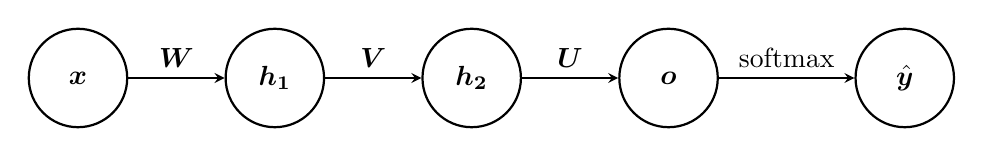
\begin{tikzpicture}[>=stealth, auto, node distance=2.5cm, semithick]
	\tikzstyle{every state}=[draw=black, thick, fill=white, minimum size=1.25cm]
	
	\node[state] (x) {$\bm{x}$};
	\node[state] (h1) [right of=x] {$\bm{h_1}$};
	\node[state] (h2) [right of=h1] {$\bm{h_2}$};
	\node[state] (o)  [right of=h2] {$\bm{o}$};
	\node[state] (y) [right of=o, node distance=3cm] {$\hat{\bm{y}}$};
	
	\path[->] (x) edge node {$\bm{W}$} (h1);
	\path[->] (h1) edge node {$\bm{V}$} (h2);
	\path[->] (h2) edge node {$\bm{U}$} (o);
	\path[->] (o) edge node {softmax} (y);
	\end{tikzpicture}
	\caption{MLP computational graph}
	\label{fig:mlp}
\end{figure}
	
Similar to the RNN, the input is defined by $\bm{x}$, the predicted label $\hat{\bm{y}}$, and the target labels $\bm{y}$. The loss function $\mathcal{L}$ is again the cross-entropy loss.\\

The rest of the graph is defined as such:
\begin{equation}
\begin{split}
	\bm{a}_1 &= \bm{W}\bm{x} + \bm{b} \\
	\bm{h}_1 &= \text{ReLU}(\bm{a}_1) \\
	\bm{a}_2 &= \bm{V}\bm{h}_1 + \bm{c} \\
	\bm{h}_2 &= \text{ReLU}(\bm{a}_1) \\
	\bm{o} &= \bm{U}\bm{h}_2 + \bm{d} \\
	\hat{\bm{y}} &= \text{softmax}(\bm{o})
\end{split}
\end{equation}

\subsubsection{Backward}
The equations for backpropagation of the MLP are defined similar to the RNN.

\paragraph{Output layer}
\begin{equation}
\begin{split}
	\frac{\partial\mathcal{L}}{\partial\bm{o}}
		&= \text{softmax}(\bm{o} - \bm{y}) \\
		&= \hat{\bm{y}} - \bm{y}
\end{split}
\end{equation}

\begin{equation}
\begin{split}
	\frac{\partial\mathcal{L}}{\partial\bm{d}}
		&=	\frac{\partial\mathcal{L}}{\partial\bm{o}} \frac{\partial\bm{o}}{\partial\bm{d}} \\
		&= \frac{\partial\mathcal{L}}{\partial\bm{o}}
\end{split}
\end{equation}

\begin{equation}
\begin{split}
\frac{\partial\mathcal{L}}{\partial\bm{U}}
	&=	\frac{\partial\mathcal{L}}{\partial\bm{o}} \frac{\partial\bm{o}}{\partial\bm{U}} \\
	&= \frac{\partial\mathcal{L}}{\partial\bm{o}} \;\bm{h}_2^T
\end{split}
\end{equation}

\paragraph{Second hidden layer}
\begin{equation}
\begin{split}
	\frac{\partial\mathcal{L}}{\partial\bm{h}_2}
		&= \frac{\partial\mathcal{L}}{\partial\bm{o}} \frac{\partial\bm{o}}{\partial\bm{h}_2} \\
		&= \bm{U}^T\; \frac{\partial\mathcal{L}}{\partial\bm{o}}
\end{split}
\end{equation}

\begin{equation}
\begin{split}
	\frac{\partial\mathcal{L}}{\partial\bm{a}_2}
		&= \frac{\partial\mathcal{L}}{\partial\bm{h}_2} \frac{\partial\bm{h}_2}{\partial\bm{a}_2} \\
	\left(\frac{\partial\bm{h}_2}{\partial\bm{a}_2}\right)_i 
		&= \left\{\begin{matrix}
			1, (\bm{a}_2)_i \geq 0 \\ 
			0, (\bm{a}_2)_i < 0
			\end{matrix}\right.
\end{split}
\end{equation}

\begin{equation}
\begin{split}
	\frac{\partial\mathcal{L}}{\partial\bm{c}}
		&= \frac{\partial\mathcal{L}}{\partial\bm{a}_2} \frac{\partial\bm{a}_2}{\partial\bm{c}} \\
		&= \frac{\partial\mathcal{L}}{\partial\bm{a}_2}
\end{split}
\end{equation}

\begin{equation}
\begin{split}
	\frac{\partial\mathcal{L}}{\partial\bm{V}}
		&= \frac{\partial\mathcal{L}}{\partial\bm{a}_2} \frac{\partial\bm{a}_2}{\partial\bm{V}} \\
		&= \frac{\partial\mathcal{L}}{\partial\bm{a}_2} \;\bm{h}_1^T
\end{split}
\end{equation}

\paragraph{First hidden layer}
\begin{equation}
\begin{split}
	\frac{\partial\mathcal{L}}{\partial\bm{h}_1}
		&= \frac{\partial\mathcal{L}}{\partial\bm{a}_2} \frac{\partial\bm{a}_2}{\partial\bm{h}_1} \\
		&= \bm{V}^T\; \frac{\partial\mathcal{L}}{\partial\bm{a}_2}
\end{split}
\end{equation}

\begin{equation}
\begin{split}
	\frac{\partial\mathcal{L}}{\partial\bm{a}_1}
		&= \frac{\partial\mathcal{L}}{\partial\bm{h}_1} \frac{\partial\bm{h}_1}{\partial\bm{a}_1} \\
	\left(\frac{\partial\bm{h}_1}{\partial\bm{a}_1}\right)_i 
		&= \left\{\begin{matrix}
			1, (\bm{a}_1)_i \geq 0 \\ 
			0, (\bm{a}_1)_i < 0
			\end{matrix}\right.
\end{split}
\end{equation}

\begin{equation}
\begin{split}
	\frac{\partial\mathcal{L}}{\partial\bm{b}}
		&= \frac{\partial\mathcal{L}}{\partial\bm{a}_1} \frac{\partial\bm{a}_1}{\partial\bm{b}} \\
		&= \frac{\partial\mathcal{L}}{\partial\bm{a}_1}
\end{split}
\end{equation}

\begin{equation}
\begin{split}
	\frac{\partial\mathcal{L}}{\partial\bm{W}}
		&= \frac{\partial\mathcal{L}}{\partial\bm{a}_1} \frac{\partial\bm{a}_1}{\partial\bm{W}} \\
		&= \frac{\partial\mathcal{L}}{\partial\bm{a}_1} \;\bm{x}^T
\end{split}
\end{equation}

\subsection{Training}
\subsubsection{Weight initialization}
All weights were initialized with values sampled from a Gaussian distribution $\mathcal{N} \sim \{0, 0.1^2\}$.\\
All biases were initialized with a constant value $0.1$.

\begin{verbatim}
    W = np.random.normal(0, 0.1, size=[300, 128])
    b = np.ones(shape=[1, 128]) * 0.1
\end{verbatim}

\subsubsection{Batch updates}
The weight updates were done in batches. $b$ sentences were randomly chosen, where $b$ is a hyperparameter. The gradients of each sentence were first independently obtained. Then, the mean of those gradients were taken and applied to the weights.\\

This helped to smooth the loss decrease over training. We compare the value of the training loss over time before and after implementing batch updates in Figure \ref{fig:batch-updates}.

\begin{figure}[h]
	\centering
	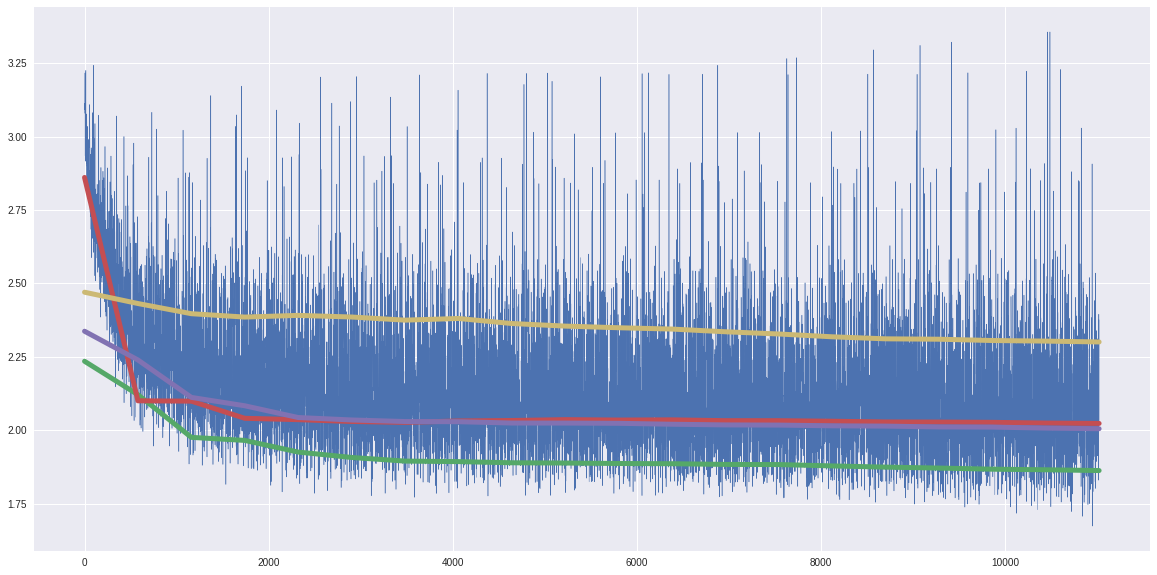
\includegraphics[width=0.45\linewidth]{assets/loss_nobatch.png}
	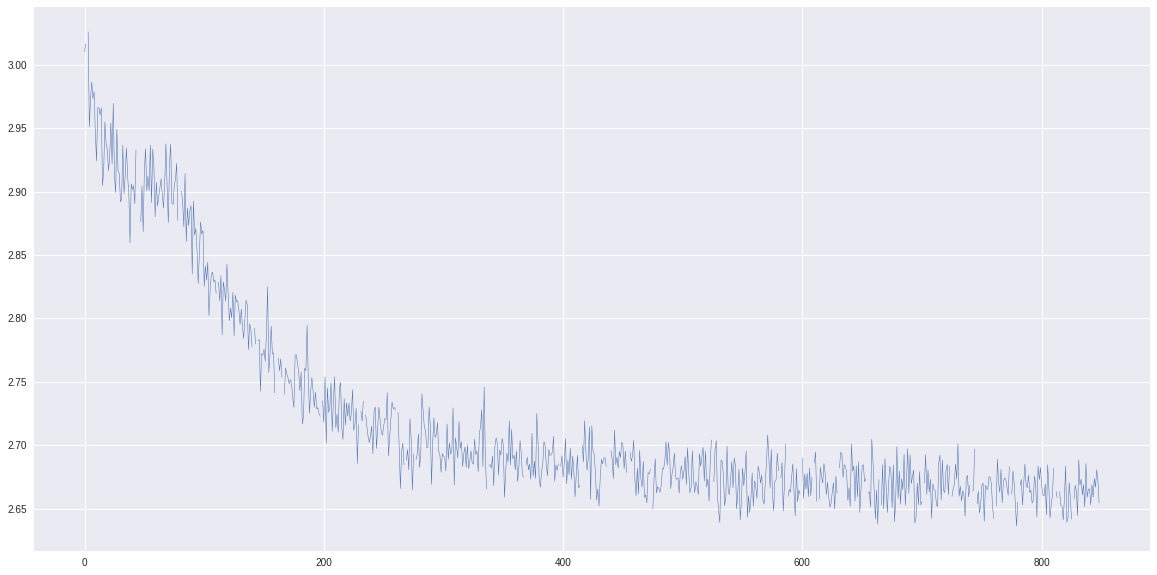
\includegraphics[width=0.45\linewidth]{assets/loss_batch.png}
	\subfloat[Before batch updates]{\hspace{0.5\linewidth}}
	\subfloat[After batch updates]{\hspace{0.5\linewidth}}
	\caption{Training loss against epochs}
	\label{fig:batch-updates}	
\end{figure}

\subsubsection{Optimizers}
\paragraph{Stochastic gradient descent}\mbox{}\\
SGD was the initial choice of optimizer due to its ease of implementation. However, it was shown to perform poorly on class imbalance without strong regularization.

\paragraph{Adagrad}\mbox{}\\
Adagrad was then used in place of SGD. This yielded highly favourable results.

\begin{verbatim}
    cum_grad = [np.zeros_like(weight) for weight in model]
    for i in range(n):
        loss, grad = backward(*model, x=x, y=y)

        # gradient accumulation
        for cum_weight, weight_update in zip(cum_grad, grad):
            cum_weight += np.square(weight_update)

        # gradient update
        for weight, cum_weight, weight_update in zip(model, cum_grad, grad):
            weight -= (lr / (np.sqrt(cum_weight) + 1e-6)) * weight_update
\end{verbatim}

\subsubsection{Regularization}
We add $L_2$ regularization to the weights $\bm{U}, \bm{W}, \bm{V}$.\\
This adds an additional term to their gradients, e.g. $\lambda \lVert\bm{U}\rVert_1$, where $\lambda$ is the regularization penalty coefficient.\\

The regularization term helped to deal with the class imbalance in the labels during training of the RNN. The class imbalance is illustrated in Figure \ref{fig:class-labels}.

\begin{figure}[h]
	\centering
	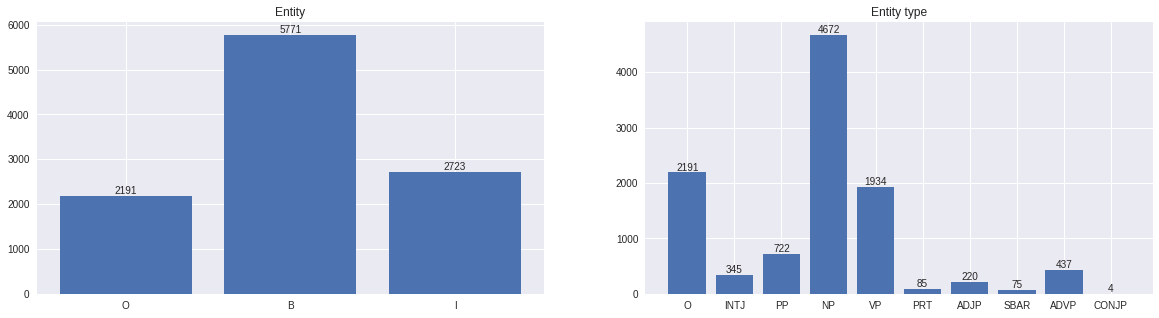
\includegraphics[width=0.9\linewidth]{assets/class_labels.png}
	\caption{Distribution of labels in FR dataset}
	\label{fig:class-labels}
\end{figure}

\subsubsection{Class weighting}
The class imbalance as illustrated in Figure \ref{fig:class-labels} caused the model to over-predict a particular class, resulting in very recall.\\

In order to correct the class imbalance, the gradient function was modified to include class weights $w$:
	$$ \frac{\partial \mathcal{L}^{(t)}}{\partial \bm{o}^{(t)}}
		= (\hat{\bm{y}}^{(t)} - \bm{y}^{(t)}) \circ w $$
where $\circ$ is the element-wise multiplication between the two vectors.\\

However, by introducing class weights, it was found that the precision of the results drastically worsened. As such, class weighting was not used.

\subsubsection{Hyperparameter optimization}

In order to determine the optimal hyperparameters for this task, we perform a grid search. We enumerate over the following hyperparameters and the possible values:
\begin{table}[htpb]
    \centering
    \begin{tabular}{|l|c|}
        \hline
        Hyperparameter & Possible Values \\ \hline
        Batch Size & [8, 16, 32, 50, 64] \\ \hline
        Learning Rate & [1e-2, 1e-3, 1e-4] \\ \hline
        Learning Rate Decay & [1.0, 0.95, 0.9] \\ \hline
        Hidden Dimension & [32, 64, 128, 256, 512] \\ \hline
    \end{tabular}
    \caption{Hyperparameter Selection}
\end{table}

After performing the above search, we selected the best results based on the validation set. These were consistent for both the FR and EN dataset, with the optimal parameters being a batch size of $32$, learning rate of $1e-2$, learning rate decay of $1.0$ (no decay), and hidden dimension of $512$. The results for this model is presented in Table \ref{table:mlpresults}.

\subsection{Results}
We compare the results on the EN and FR datasets between the RNN and MLP method.

\subsubsection{RNN}
\begin{table}[htpb]
	\centering
	\begin{tabular}{|l|c|c|}
		\hline
		\multirow{2}{*}{\textbf{Dataset}} & \multicolumn{2}{c|}{\textbf{F-Score}} \\ \cline{2-3} 
		& \multicolumn{1}{l|}{\textbf{Entity}} & \multicolumn{1}{l|}{\textbf{\begin{tabular}[c]{@{}l@{}}Entity\\ Type\end{tabular}}} \\ \hline
		EN & 0.572 & 0.268 \\ \hline
		FR & 0.136 & 0.094 \\ \hline
	\end{tabular}

    \caption{RNN Results}
\end{table}

\subsubsection{MLP}
\begin{table}[htpb] 
	\centering
	\begin{tabular}{|l|c|c|}
		\hline
		\multirow{2}{*}{\textbf{Dataset}} & \multicolumn{2}{c|}{\textbf{F-Score}} \\ \cline{2-3} 
		& \multicolumn{1}{l|}{\textbf{Entity}} & \multicolumn{1}{l|}{\textbf{\begin{tabular}[c]{@{}l@{}}Entity\\ Type\end{tabular}}} \\ \hline
		EN & 0.700 & 0.614 \\ \hline
		FR & 0.677 & 0.467 \\ \hline
	\end{tabular}
    \caption{MLP Results}
    \label{table:mlpresults}
\end{table}

\subsection{Evaluation}

In general, we see that the MLP performs significantly  better than the RNN on all metrics. This is likely due to the vanishing gradients problem of the RNN, as some of the sentences may be quite long. Additionally, the FR dataset is quite poorly labeled, with most of the words being designated a label of "O". This may point to the downsides of a sequence based model, which may overfit to the poor structure in the sentences. We attribute the performance gain of the MLP for this task due to its high fitting power. With a hidden dimension size of $512$ neurons, it is able to fit the training set very well. \\

To counter overfitting, we initially tried several regularization techniques such as dropout and weight decay. However, this did not have a noticeable improvement on the validation score. We think this may be due to the training and validation set having similar data distributions. Hence, our model is able to generalize well to the validation set.


\newpage
\bibliographystyle{ieeetr}
\bibliography{bibliography}

\end{document}
